\section{Retrospettiva}
%Restrospettiva (descrizione finale dettagliata dell'andamento dello sviluppo, del backlog, delle iterazioni; commenti finali)
%Si noti che la retrospettiva è l'unica sezione che può citare aneddoti di cosa è successo in itinere, mentre le altre sezioni fotografino il risultato finale. Se gli studenti decideranno (come auspicato) di utilizzare un product backlog e/o dei backlog delle varie iterazioni/sprint, è opportuno che questi siano file testuali tenuti in versione in una cartella "process", così che sia ri-verificabile a posteriori la storia del progetto.

\subsection{Sprint 1 27/09 - 03/10}
\paragraph{Epic} Visualizzare il personaggio a schermo

Il primo sprint è stato prevalentemente organizzativo ed è stato focalizzato sulla scelta e il setup degli strumenti, la definizione del processo di sviluppo e il design architetturale. 
In particolare si è scelto di lavorare con il framework Indigo e si è studiata la sua documentazione, al fine di comprendere come organizzare il codice e poter definire l’architettura generale del gioco. 
Era previsto anche il setup della CI/CD, abbiamo deciso però di spostarla nella seconda sprint, la quale sarà orientata a implementare la struttura base e produrre la prima schermata di gioco. 


\begin{figure}[!hbt]
    \centering
    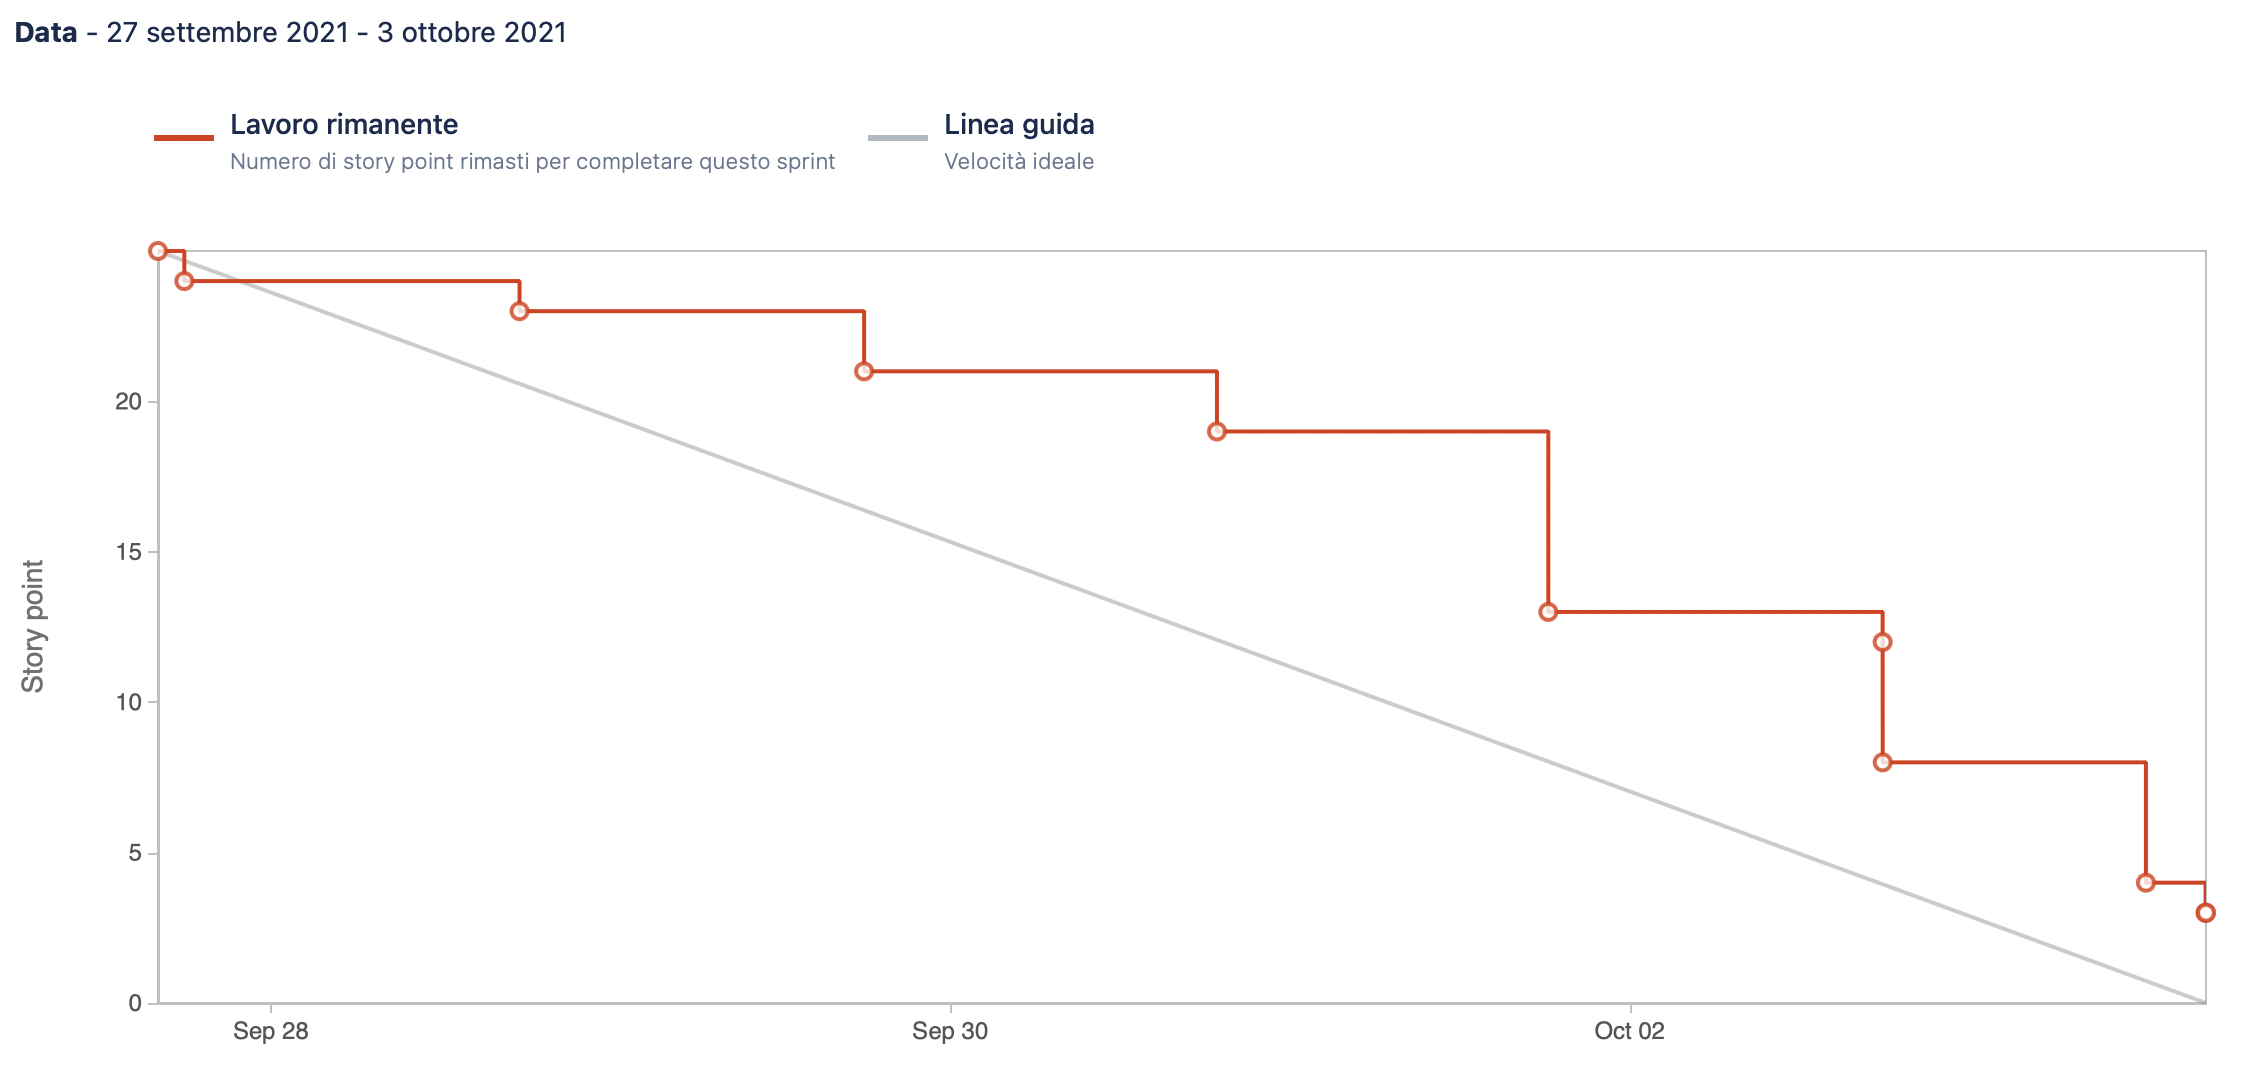
\includegraphics[scale=0.35]{sprint-1-burn-down.png}
    \caption{\textit{Grafico Burn-down primo sprint}} 
\end{figure}


\subsection{Sprint 2 04/10 - 10/10}
\paragraph{Epic} Visualizzare il personaggio a schermo

Nel secondo sprint abbiamo effettuato il setup dell'architettura includendo Indigo, al fine di visualizzare il menu di avvio, il loading e permettere all'utente di visualizzare il proprio personaggio all'interno di una stanza vuota. 
Abbiamo inoltre abilitato la continuous integration. Siamo così giunti all'obbiettivo dell'epic. In questa sprint, abbiamo fatto i primi passi con l'engine Indigo, confrontandoci costantemente in modo da sperimentare insieme il suo utilizzo. Questo ci ha permesso di allineare la nostra conoscenza a riguardo e definire una modalità operativa per le future sprint. 
Non siamo riusciti a completare la visualizzazione del personaggio in quanto ci siamo resi conto di dover impostare meglio il modello generale al fine di realizzare una struttura a componenti che funzioni con Indigo.

\begin{figure}[!hbt]
    \centering
    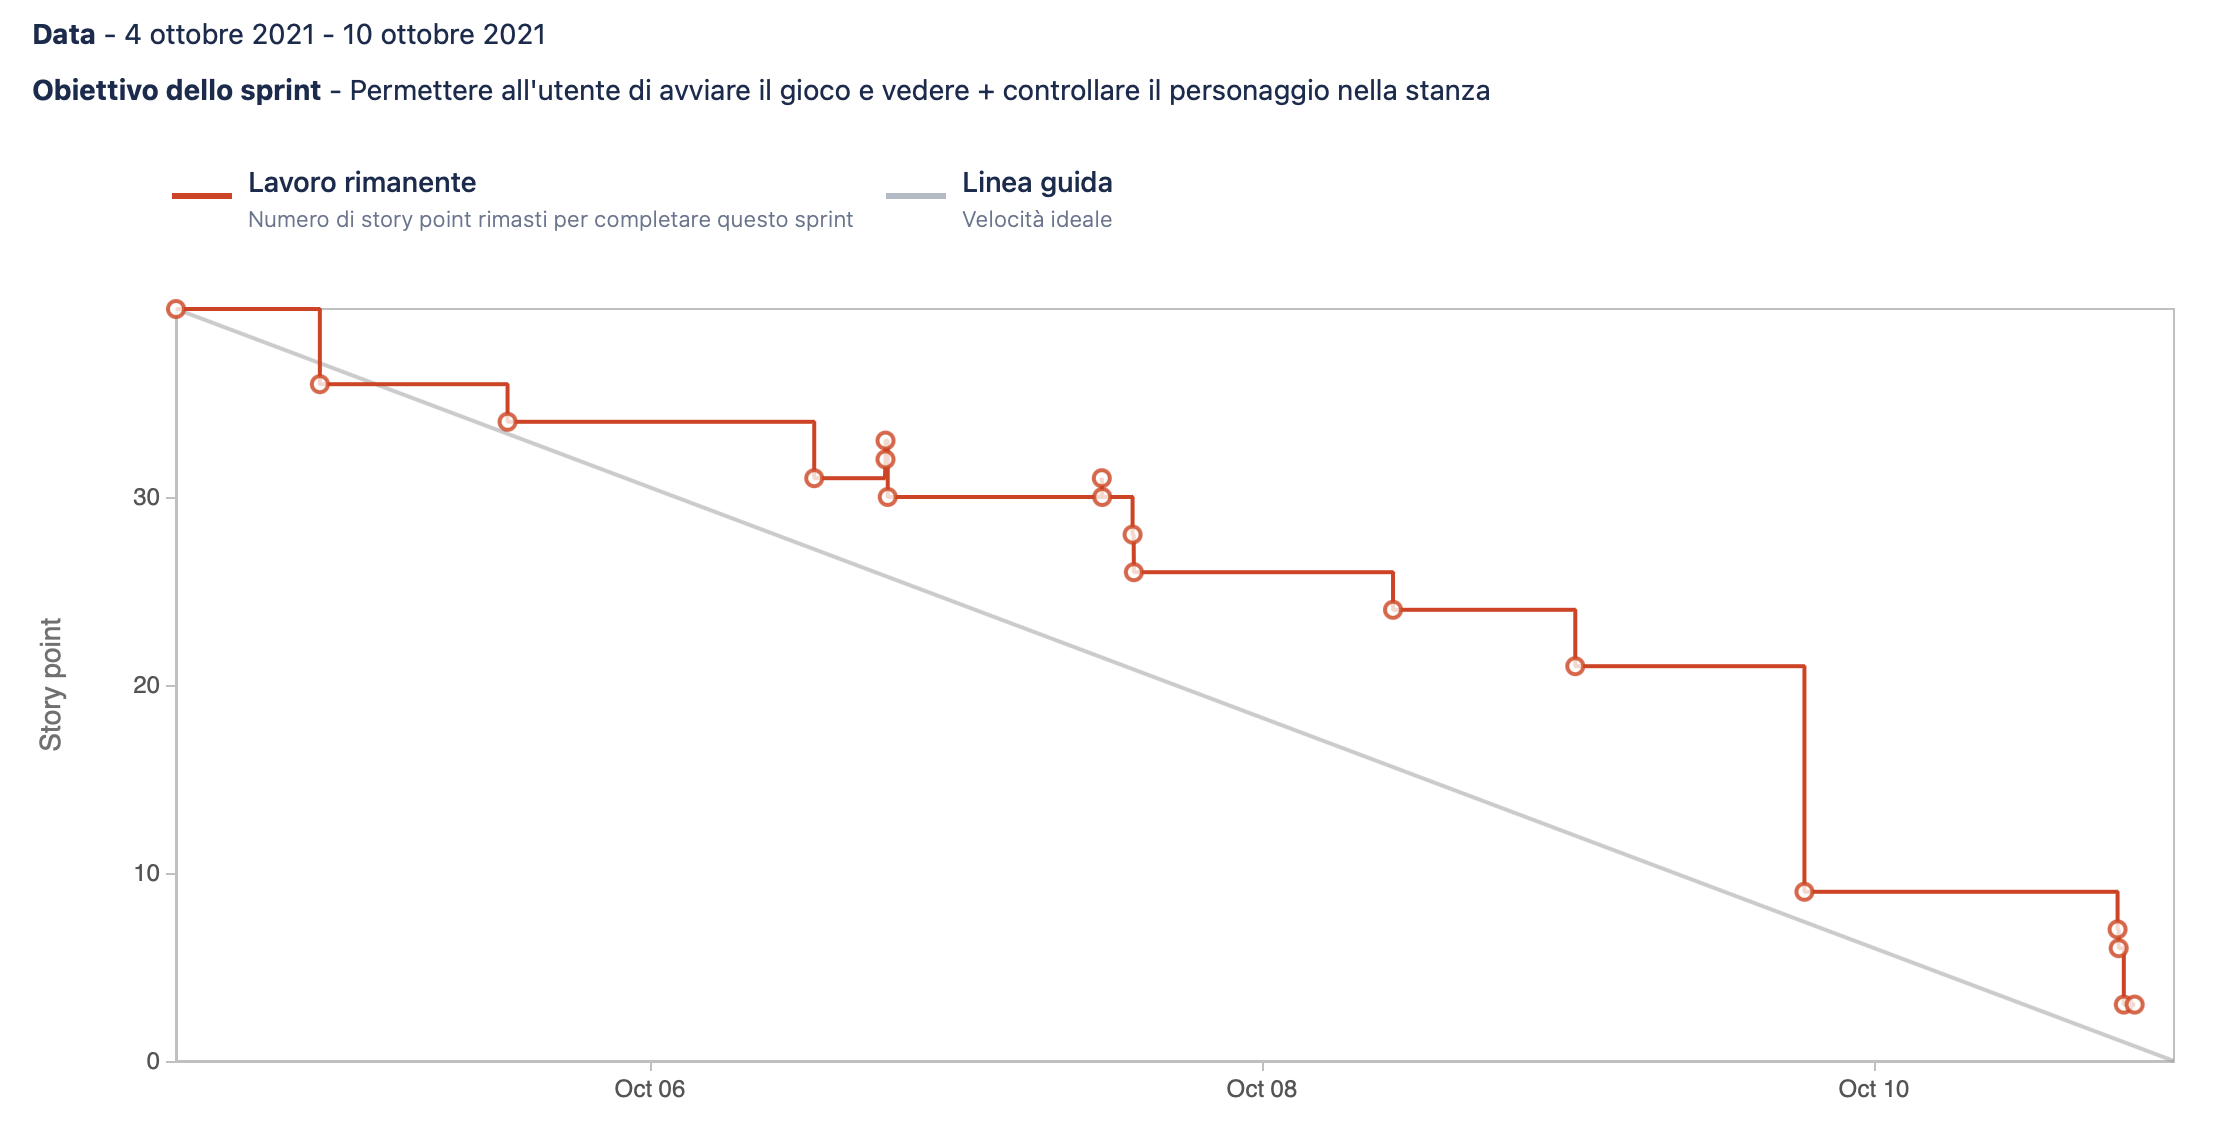
\includegraphics[scale=0.35]{sprint-2-burn-down.png}
    \caption{\textit{Grafico Burn-down secondo sprint}} 
\end{figure}


\subsection{Sprint 3 11/10 - 17/10}

Il terzo sprint è stato dedicato al rifinimento del personaggio aggiungendo animazioni e vincolandolo all'interno dei confini della stanza. 
Questo ha richiesto di approfondire lo studio di Indigo riguardo le animazione e rifattorizzare la stanza, le sue proprietà e la sua logica. 
Oltre a questo è stata rivista la gerarchia di classi che supportano il personaggio e che sarà alla base di tutti gli elementi presenti dentro alla stanza (nemici, oggetti, elementi bloccanti).
Infine, con lo studio di un workflow di test per Indigo, ci siamo predisposti per uno sviluppo TDD che avverrà dalle prossime sprint.


\begin{figure}[!hbt]
    \centering
    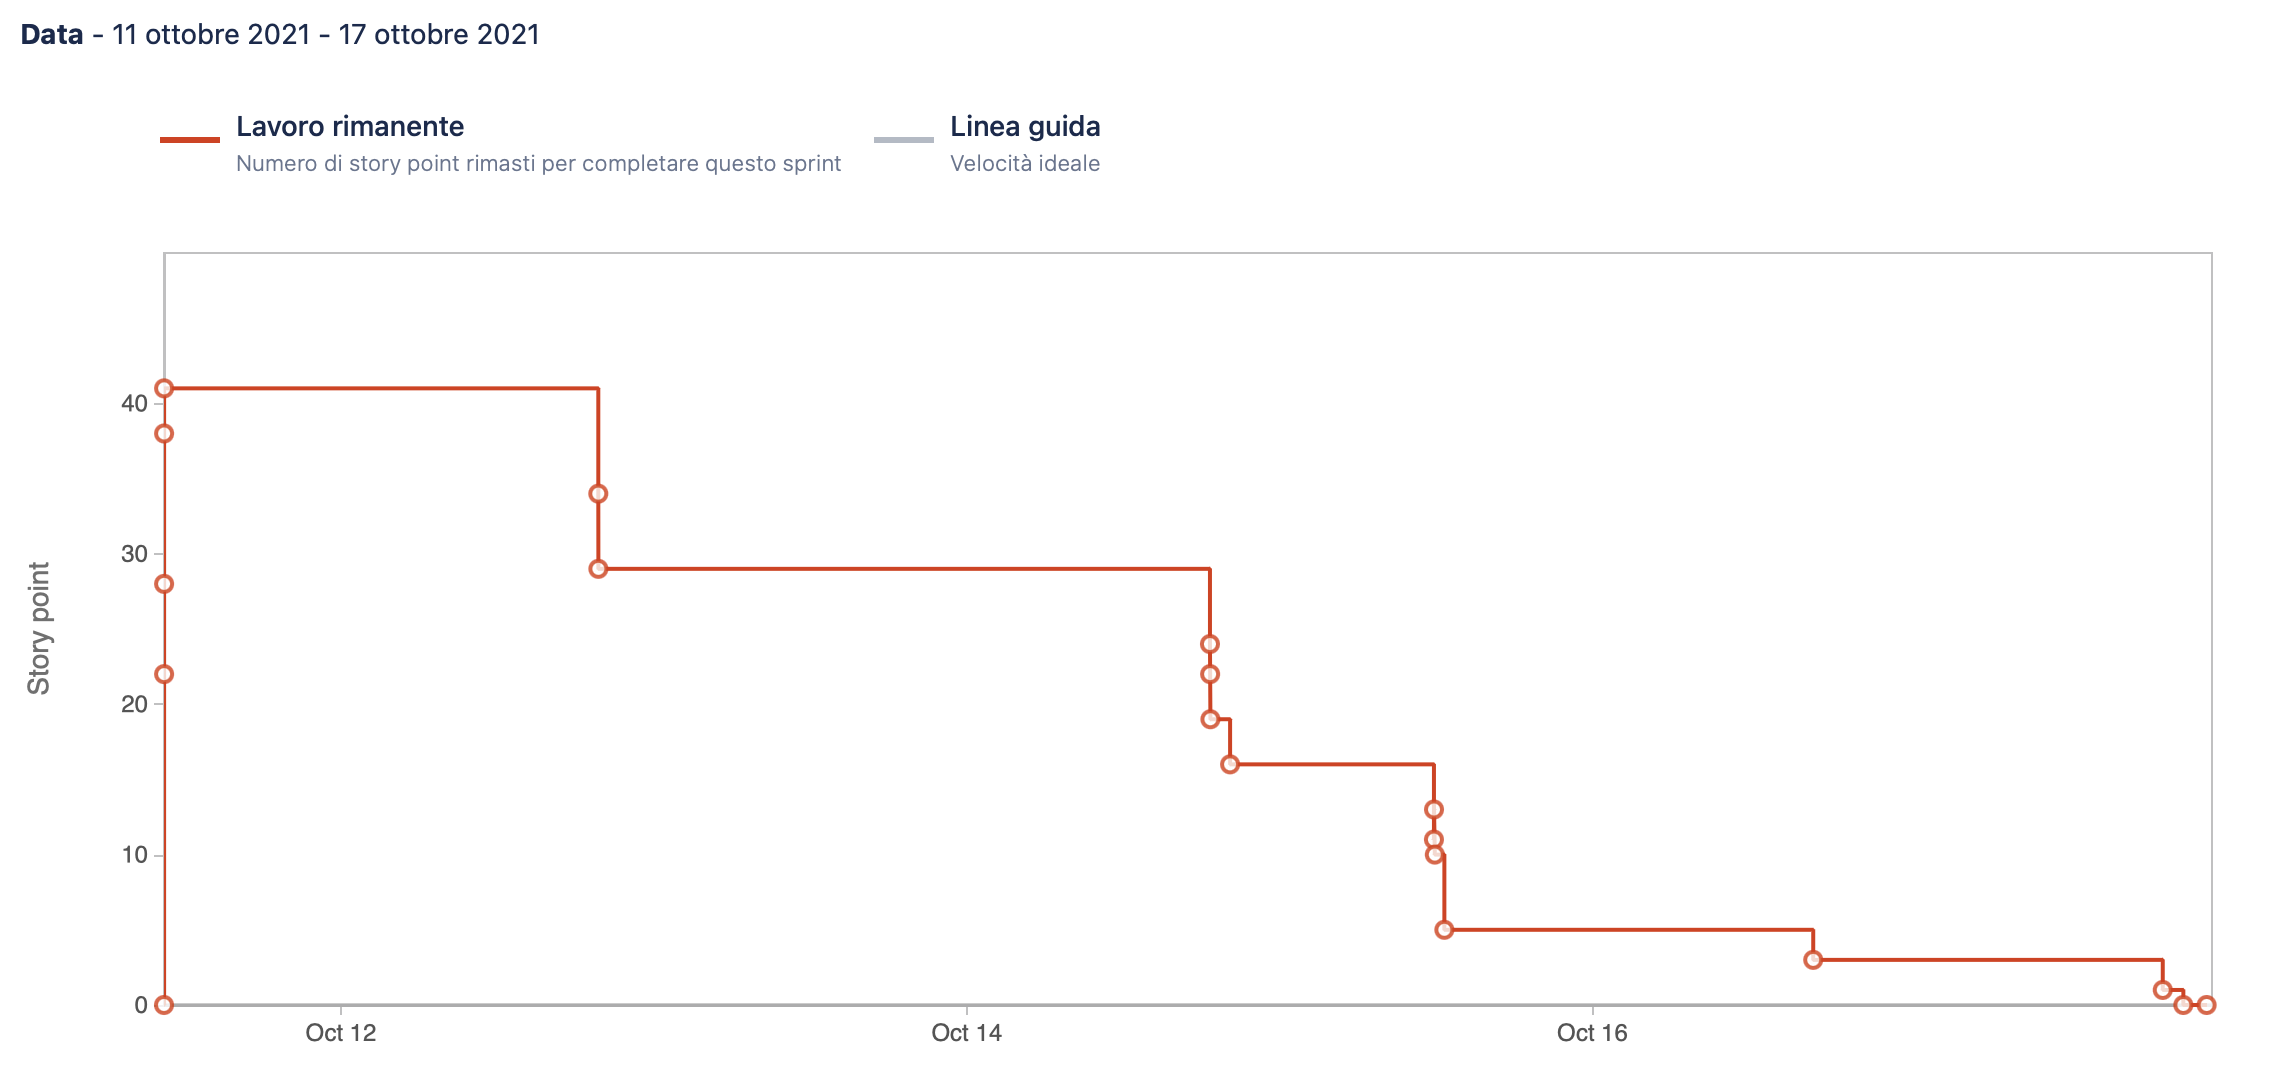
\includegraphics[scale=0.35]{sprint-3-burn-down.png}
    \caption{\textit{Grafico Burn-down terzo sprint}} 
\end{figure}

\subsection{Sprint 4 18/10 - 24/10}
Il quarto sprint è stato incentrato principalmente sul dungeon e sulla feature dello sparo per il personaggio controllato dall'utente. 
In particolare, per quanto riguarda il dungeon, è stata implementata la generazione tramite prolog e, inoltre, la possibilità di navigare tra le stanze attraverso l'uso di porte. 
Essendo Indigo basato su Scala.js abbiamo integrato un engine Prolog scritto in javascript e creato un'interfaccia in Scala per interagirvi.

Nella prossima sprint, sarà necessario un refactor e una forte integrazione tra le parti sviluppate individualmente dai diversi componenti del team.

\begin{figure}[!hbt]
    \centering
    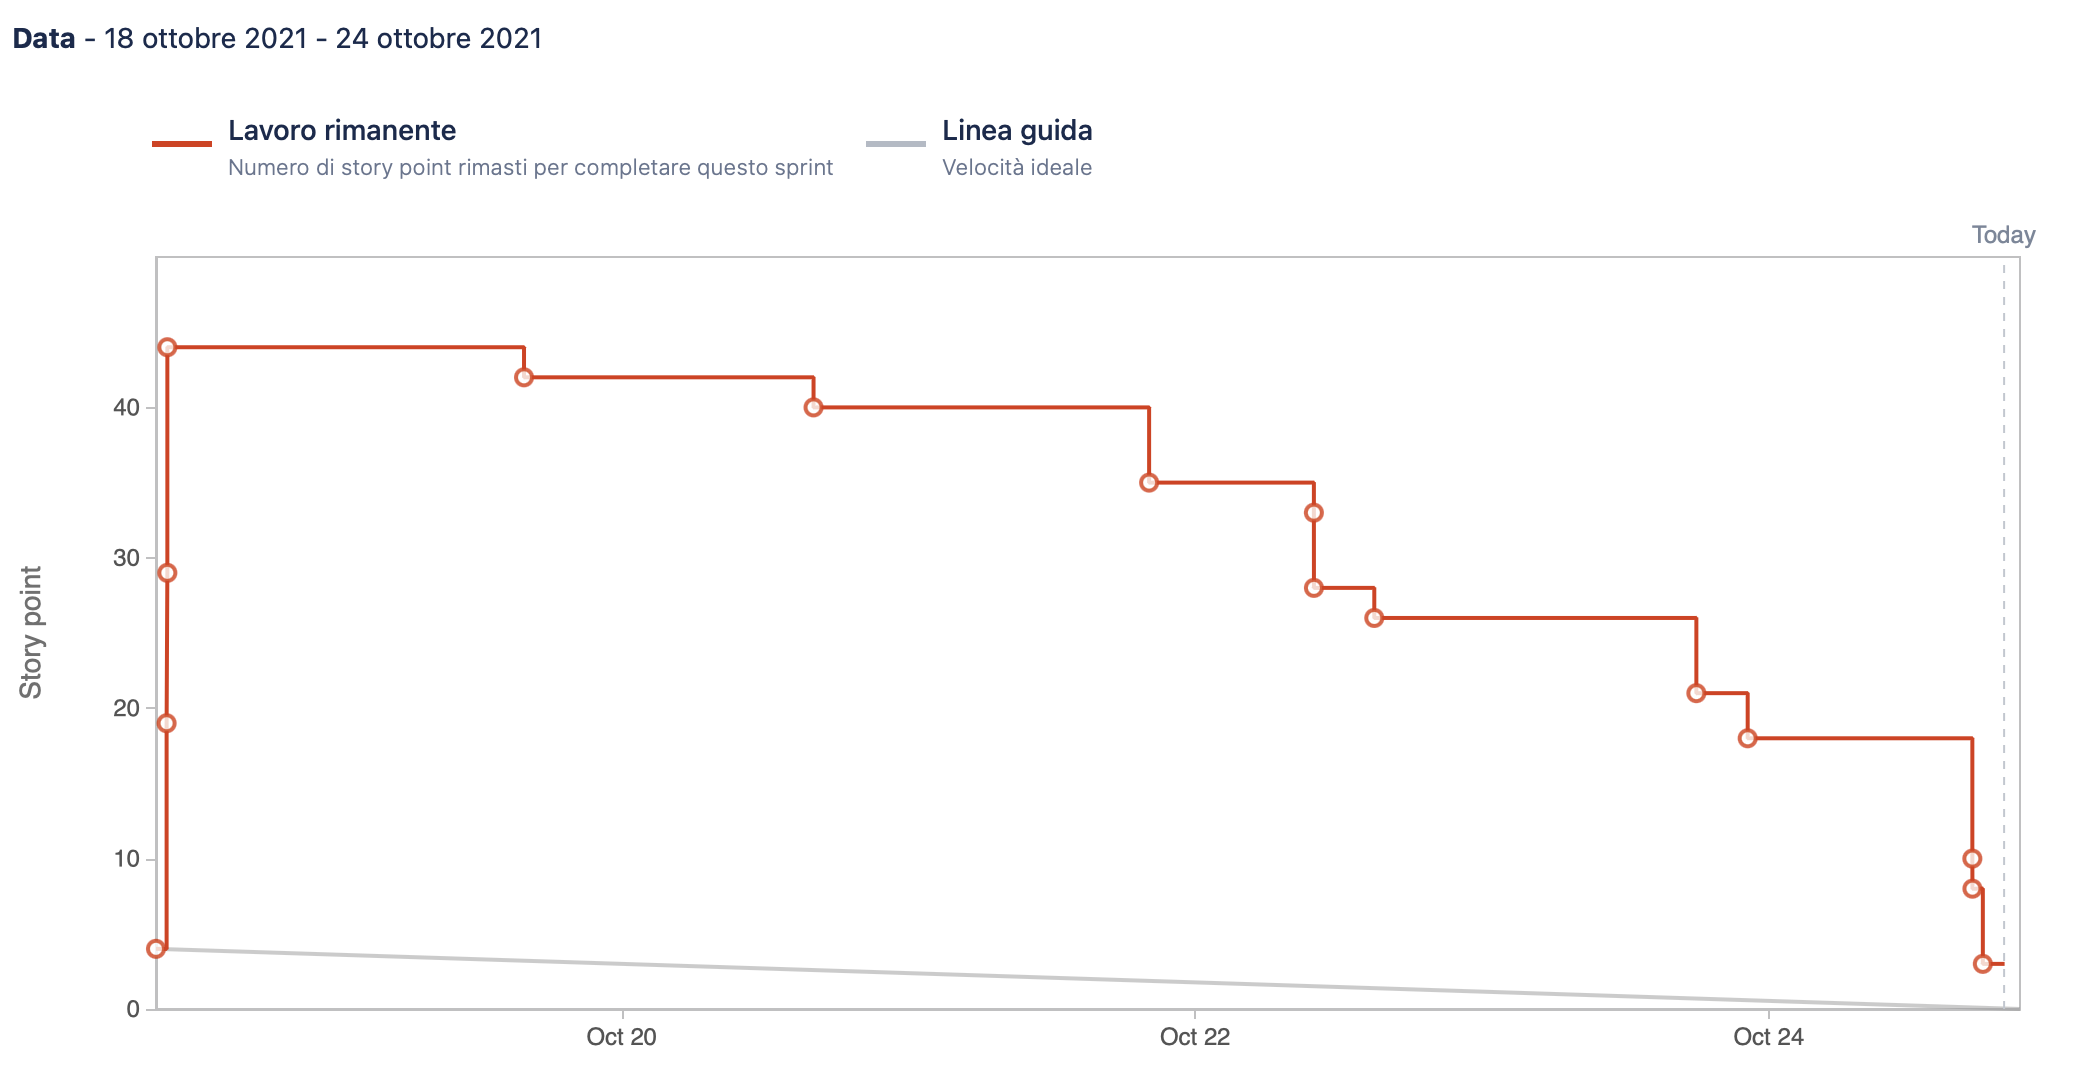
\includegraphics[scale=0.4]{sprint-4-burn-down.png}
    \caption{\textit{Grafico Burn-down quarto sprint}} 
\end{figure}


\subsection{Sprint 5 25/10 - 31/10}
Il quinto sprint è stato dedicato al refactor di diversi sezioni dell'applicativo, per permettere, nelle prossime sprint, di implementare in maniera più semplice le feature rimanenti.  
In particolare, Alan si è occupato dell'interazione Scala Prolog, in modo tale da poter utilizzare il Prolog anche per la generazione degli elementi delle stanze. Federico invece si è occupato delle Room, in modo da poter implementare le collisioni tra oggetti in maniera corretta nella prossima sprint. 
A livello di feature, all'interno di questa sprint si è dotato l'applicativo di una vera generazione casuale del dungeon e Matteo si è dedicato a dotare il personaggio di caratteristiche migliorabili. 
In questa sprint volevamo offrire più valore al committente, ma abbiamo riscontrato problemi con i test in quanto lavorando con Scala3, ScalaJS e Indigo siamo stati vincolati nella scelta dei framework di test da utilizzare. In particolare al momento non è possibile abilitare il Coverage.


\begin{figure}[!hbt]
    \centering
    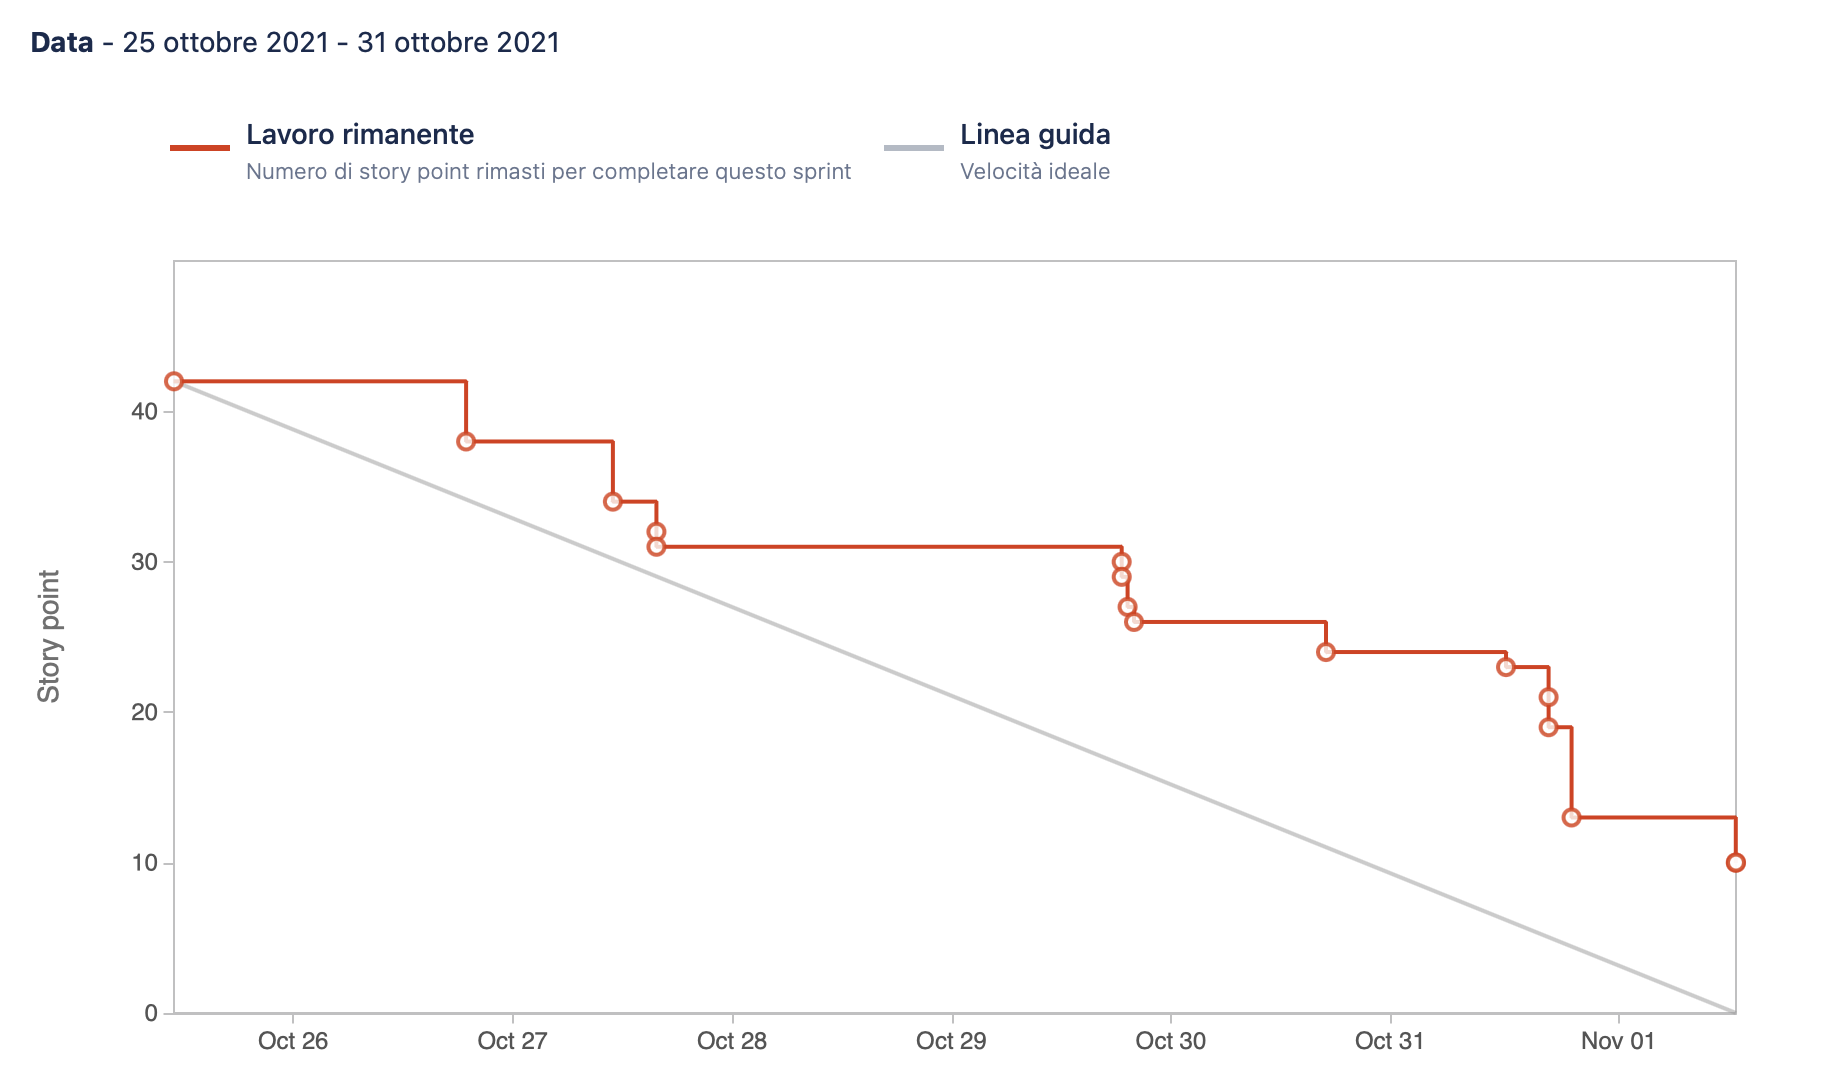
\includegraphics[scale=0.4]{sprint-5-burn-down.png}
    \caption{\textit{Grafico Burn-down quinto sprint}} 
\end{figure}

\subsection{Sprint 6 01/11 - 07/11}
Il sesto sprint è stato incentrato nel creare le dinamiche di gioco, tra cui la rilevazione delle collisioni tra gli elementi, la creazione di diversi nemici con diversi comportamenti e statiche, la visualizzazione dello stato del personaggio. 
Durante lo sprint planning abbiamo sottostimato l'effort richiesto per l'inserimento degli elementi bloccanti, anche considerando l'utilizzo del Prolog per la loro disposizione, questo richiede una nuova sprint per essere portato a termine. Un altro imprevisto è stato il dover gestire il view model per i nemici, il tutto dovuto anche a dei limiti dei Indigo, il quale non è ancora maturo a livello di engine. Anche quest'ultima parte va rifattorizzata nel prossimo sprint.
\begin{figure}[!hbt]
    \centering
    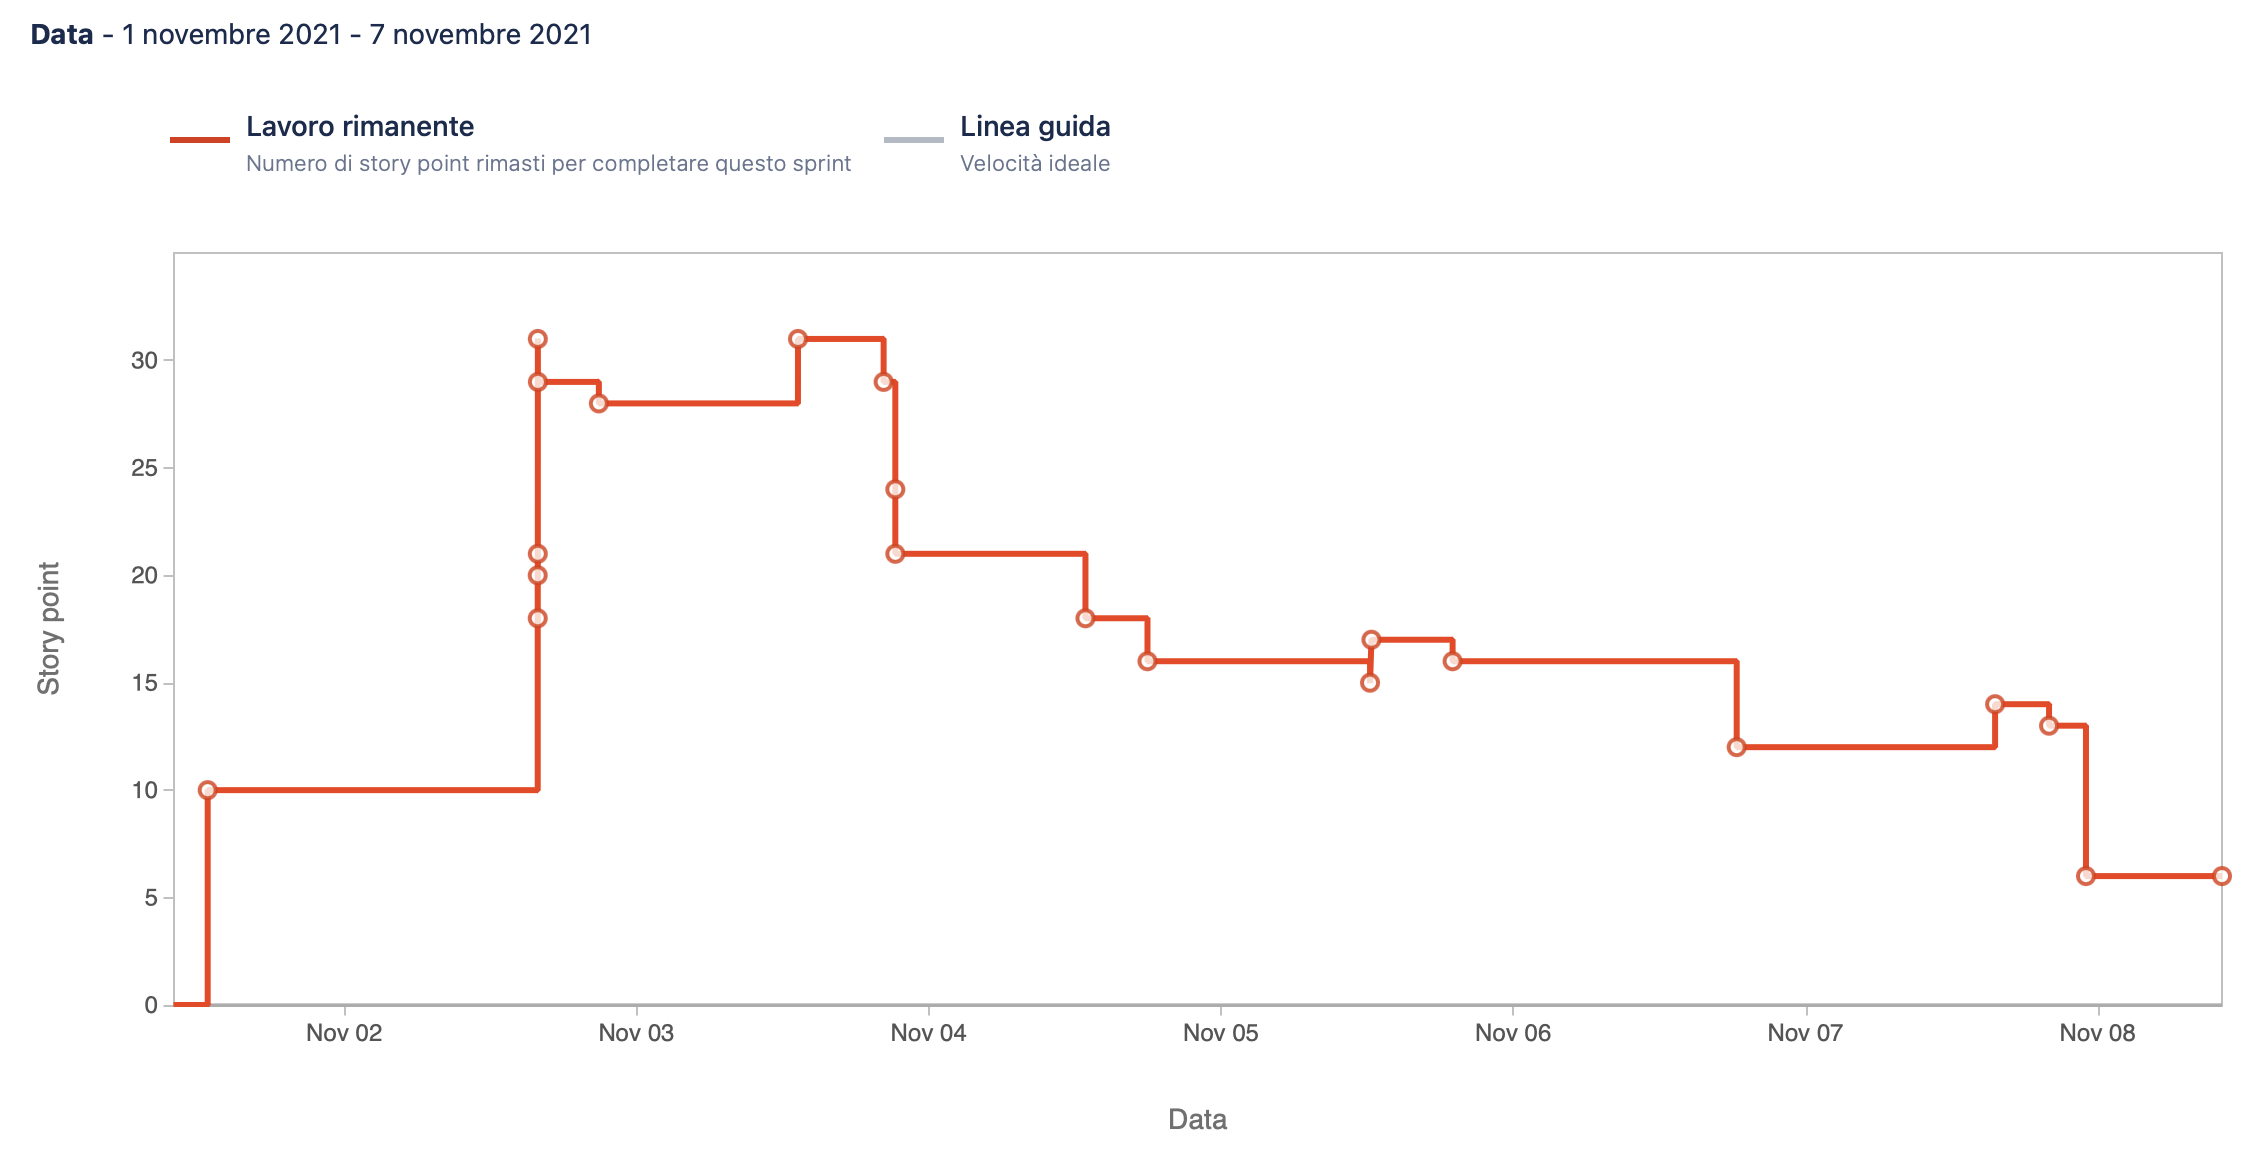
\includegraphics[scale=0.35]{sprint-6-burn-down.png}
    \caption{\textit{Grafico Burn-down sesto sprint}} 
\end{figure}

\subsection{Sprint 7 08/11 - 14/11}
Il settimo sprint è stato dedicato al refinement di alcuni punti degli sprint precedenti e all'introduzione di nuove feature, tra cui lo sviluppo ulteriore delle dinamiche di gioco e d'interazione tra il personaggio e i nemici. 
Si è quindi sviluppato un modello per le statistiche di qualsiasi elemento "Alive" e un modello di individuazione e gestione delle collisioni. 
Per quanto riguarda i refinement invece, si è ripensato all'interazione tra Model, View e ViewModel, rifattorizzando l'architettura. 
Durante questa sprint non si è ancora riusciti a concludere il posizionamento degli elementi bloccanti in Prolog per via dello sviluppo di altre feature più prioritarie.
\begin{figure}[!hbt]
    \centering
    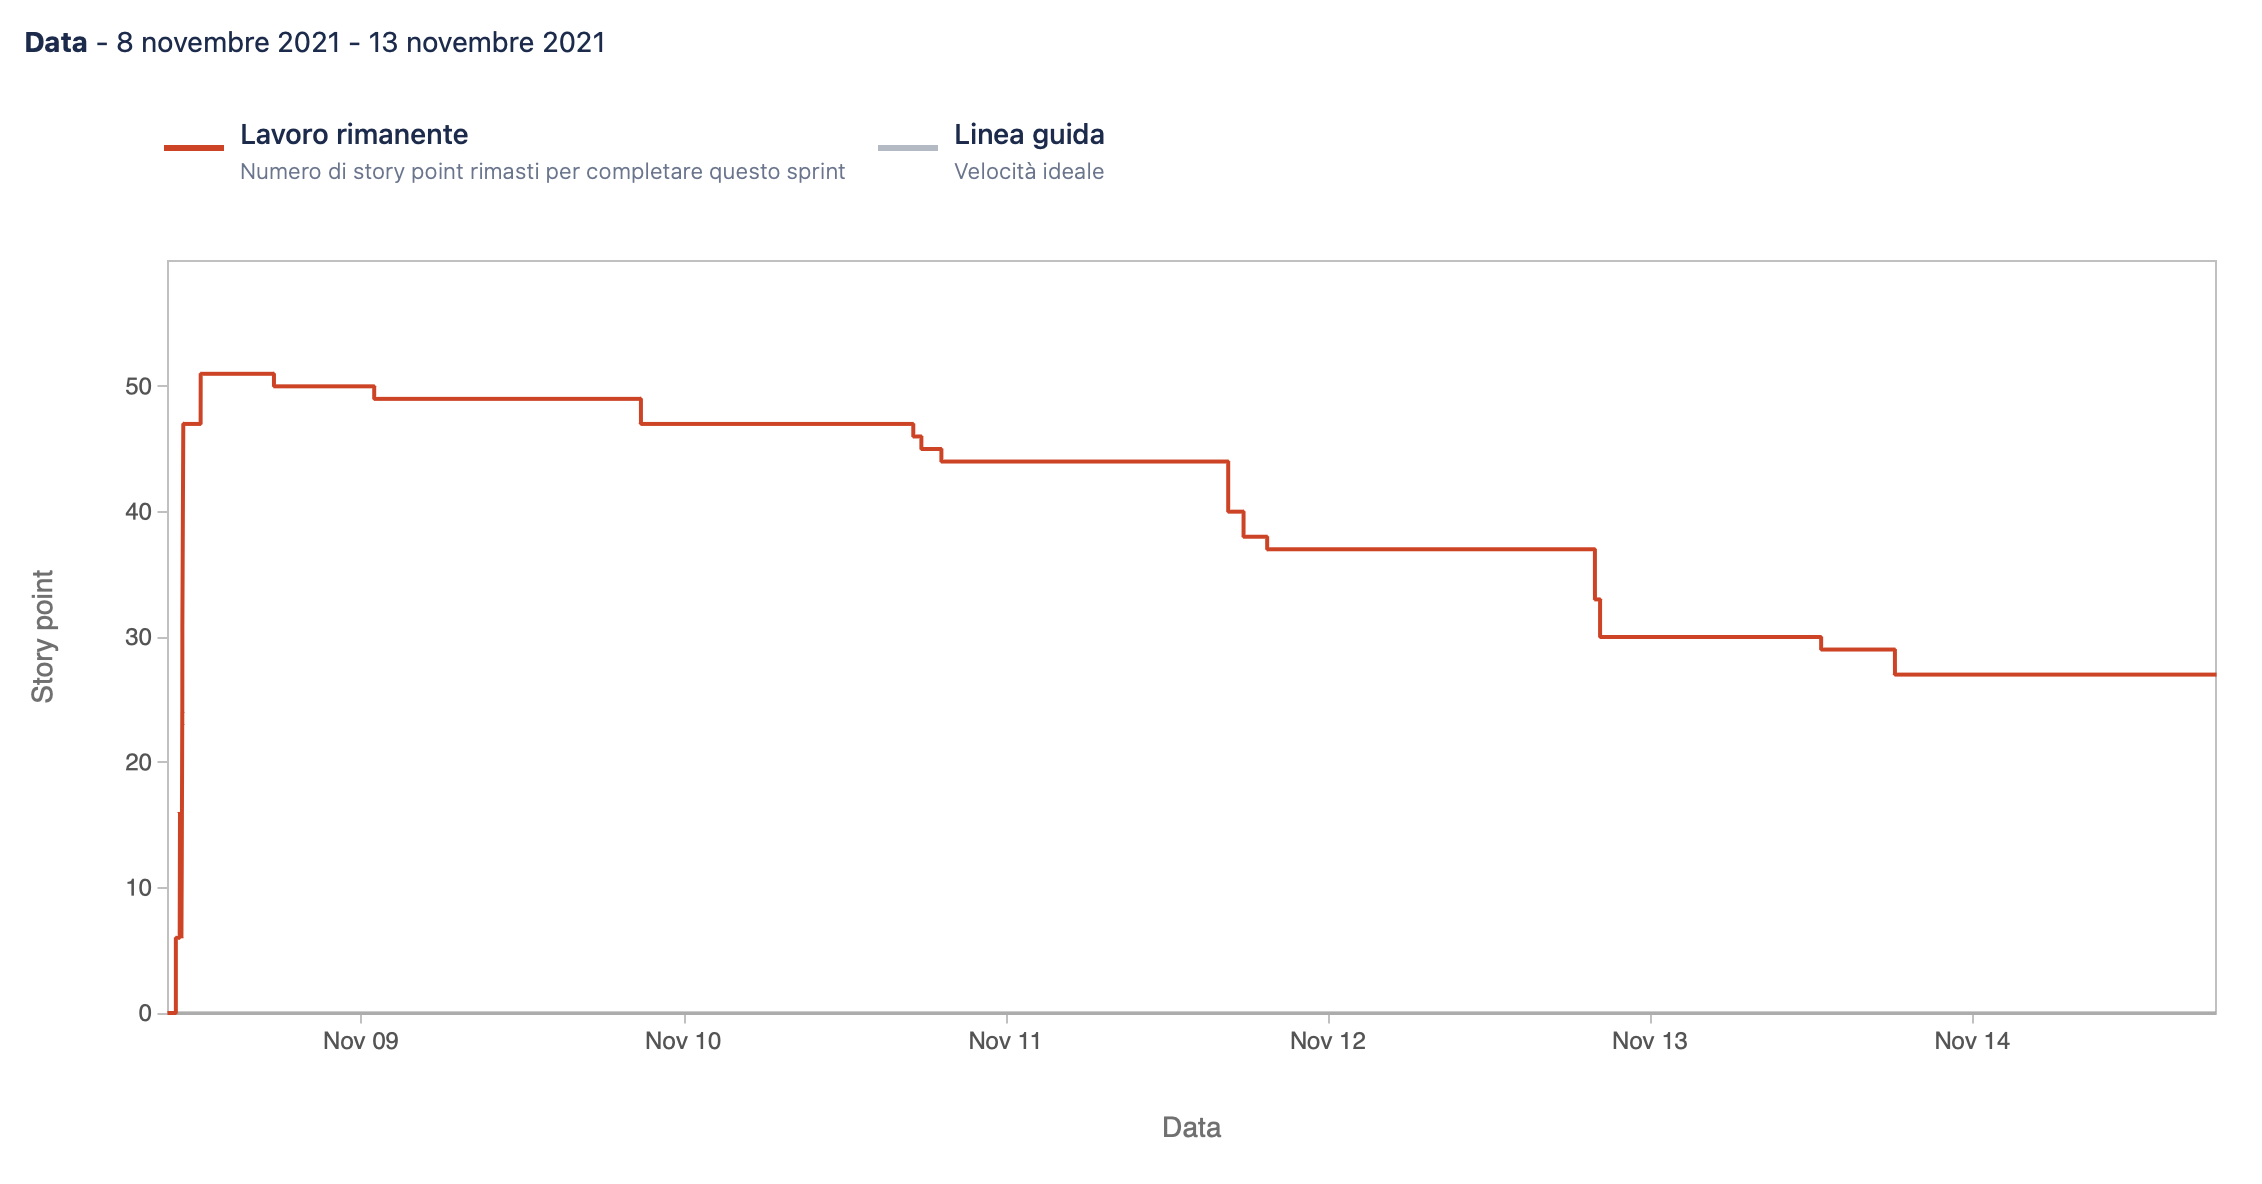
\includegraphics[scale=0.35]{sprint-7-burn-down.png}
    \caption{\textit{Grafico Burn-down settimo sprint}} 
\end{figure}


\subsection{Sprint 8 15/11 - 21/11}
A livello di feature, sono stati aggiunti alcuni elementi di valore per il gioco. 
In particolare, si è dotata la schermata di gioco di una minimappa, in modo tale che l'utente possa visualizzare a video la sua posizione nel dungeon al momento. 
Si è sviluppato un algoritmo Prolog per generare un area di gioco e un area di elementi, 
in modo tale da poter disporre all'interno della stanza nemici ed elementi bloccanti in maniera consona con quanto riportato nei requisiti.
Si è poi incrementato il modello delle stats in maniera tale da poter essere modificate in base ad avvenimenti accaduti durante il gioco. 
La disposizione degli elementi bloccanti necessiterà di sviluppo anche durante la prossima sprint, in particolare per quanto riguarda l'integrazione tra Prolog e Scala. 
\begin{figure}[!hbt]
    \centering
    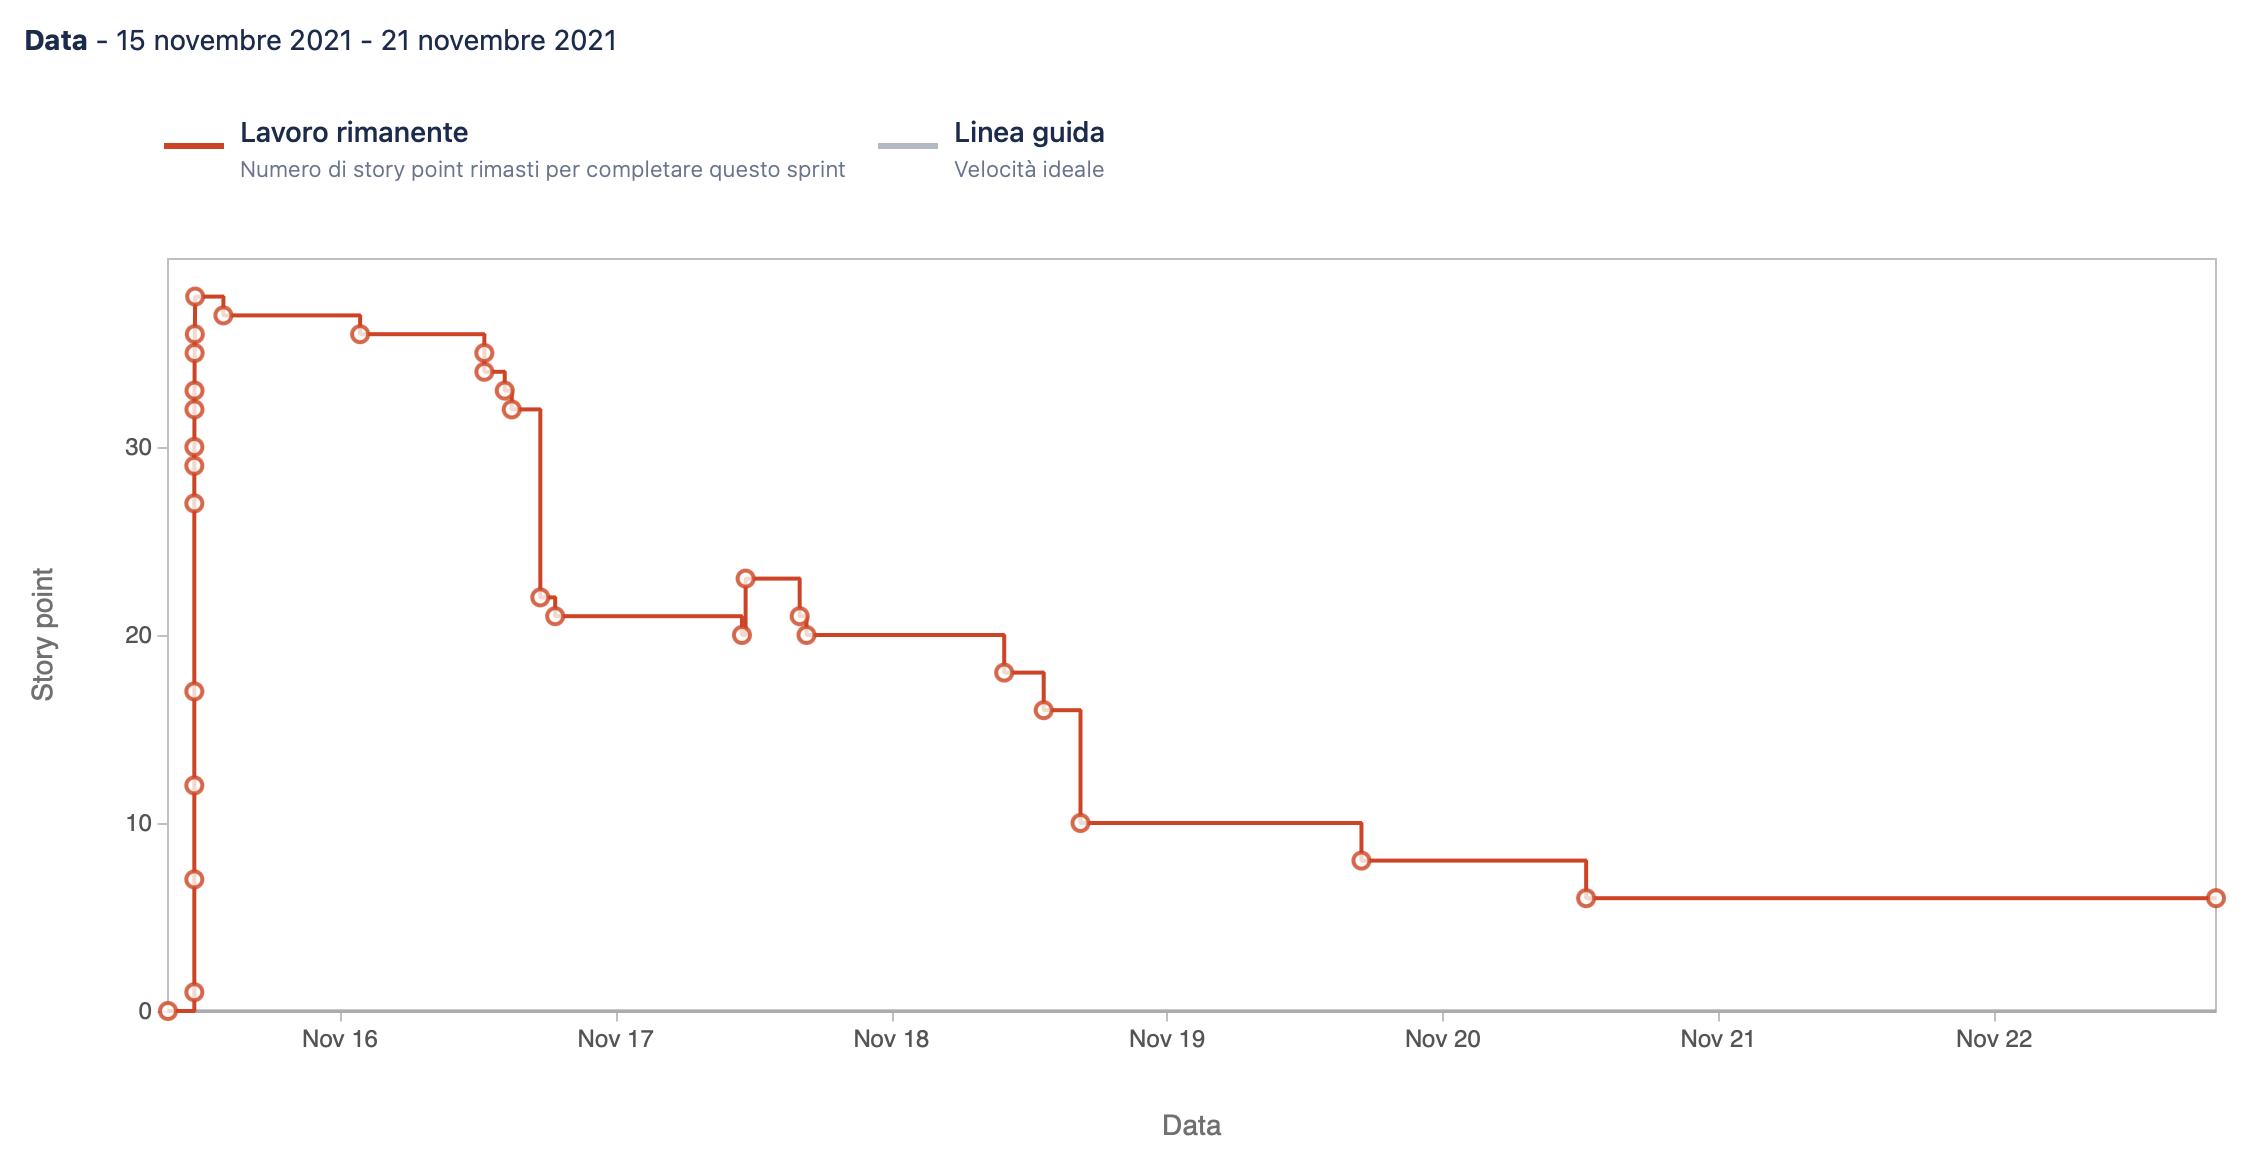
\includegraphics[scale=0.35]{sprint-8-burn-down.png}
    \caption{\textit{Grafico Burn-down ottavo sprint}} 
\end{figure}

\subsection{Sprint 9 22/11 - 28/11}